\documentclass[12pt]{article}
\usepackage{amsmath}
\usepackage{amssymb}
\usepackage{amsthm}
\usepackage{float}
\usepackage{subcaption}
\usepackage{caption}
\usepackage{graphicx}
\providecommand{\abs}[1]{\lvert#1\rvert}
\providecommand{\norm}[1]{\lVert#1\rVert}

\newtheorem{thm}{Theorem}
\newtheorem{lemma}[thm]{Lemma}
\newtheorem{fact}[thm]{Fact}
\newtheorem{cor}[thm]{Corollary}
\newtheorem{eg}{Example}
\newtheorem{ex}{Exercise}
\newtheorem{defi}{Definition}
\newtheorem{hw}{Problem}
\newenvironment{sol}
  {\par\vspace{3mm}\noindent{\it Solution}.}
  {\qed}

\newcommand{\ov}{\overline}
\newcommand{\cb}{{\cal B}}
\newcommand{\cc}{{\cal C}}
\newcommand{\cd}{{\cal D}}
\newcommand{\ce}{{\cal E}}
\newcommand{\cf}{{\cal F}}
\newcommand{\ch}{{\cal H}}
\newcommand{\cl}{{\cal L}}
\newcommand{\cm}{{\cal M}}
\newcommand{\cp}{{\cal P}}
\newcommand{\cz}{{\cal Z}}
\newcommand{\eps}{\varepsilon}
\newcommand{\ra}{\rightarrow}
\newcommand{\la}{\leftarrow}
\newcommand{\Ra}{\Rightarrow}
\newcommand{\dist}{\mbox{\rm dist}}
\newcommand{\bn}{{\mathbf N}}
\newcommand{\bz}{{\mathbf Z}}

\setlength{\parindent}{0pt}
%\setlength{\parskip}{2ex}
\newenvironment{proofof}[1]{\bigskip\noindent{\itshape #1. }}{\hfill$\Box$\medskip}

\usepackage{enumerate,fullpage,proof,color}
\newcommand{\Infer}[2]{\vcenter{\infer{#2}{#1}}}
\newcommand{\InferN}[3]{\vcenter{\infer[#3]{#2}{#1}}}

\begin{document}

\title{\huge\textbf{\ \\ \ \\Image In-painting}\vspace{11cm}}
\author{	
	\large
	Course: Software Engineering\ \ \ \ \ \ \  \ \  \  \  \ \ \ \ \ \  \ \ \ \ \\
	\ \ \ \ \ \ \ \ \ \ \ Group Member: Hu Hu \ mihawkhu@gmail.com\ \ \ \ \ \ \ \ \ \\
	\ \ \ \ \ \ \ \ \  \ \ \ \ \ \ \ \ \ \ \ \ \ \ \ \ \ \ \ \ \ \ \ \ \ Yesheng Ma \ kimi.ysma@gmail.com \\
	\ \ \ \ \ \ \ \ \  \ \ \ \ \ \ \ \ \ \ \ \ \ \ \ \ \ \ \ \ \ \   \ Yikai Zou \ zouyikai1014@163.com\\
	Instructor: Bin Sheng \ \ \ \ \ \ \ \  \ \ \ \ \ \ \ \ \ \ \ \ \ \ \  \ \ \ \ \ \ \ \\
	Project Period: 9/2016 - 12/2016\ \ \ \ \  \ \ \ \ \ \ \ \ \ \ 	
	} \date{ }

\maketitle\thispagestyle{empty}
\newpage
\tableofcontents\thispagestyle{empty}
\newpage




\section{Background and Analysis of the Problem}
Several techniques that former researchers has developed includes:
\begin{enumerate}[1.]
	\item Partial Differential Equation (PDE) based algorithm is iterating and propagating information about the graph to restore the graph.
	\item Texture synthesis based Image In-painting is to to produce more of that texture
	\item Wavelet Transform in two dimensions based in-paintinging algorithms to fix images
	\item Semi-automatic and fast in-paintinging fixes the graph with the help of human assistance.
	\item Using Markov random fields (MRF) to model the image and do image in-paintinging based on Bayesian learning in acyclic graphs.
\end{enumerate}
Problems in these image in-paintinging algorithms are that there is no universal and 
efficient algorithms to solve all kinds of image in-paintinging problems.
All currently available algorithms are all limited to a specific area of image
in-paintinging, for example text in-paintinging.


\section{Proposed Goal, Objectives, Target Population}
\subsection{Goal}
\qquad This project managed to implement the image in-painting algorithm which is mentioned in previous papers. We will try to solve the problem that they meet and give the better method to do the image in-painting. The proposed goal is that when given a picture and a chosen area, ie, draw a area on smart phone. Then we will remove the object in this area and inpaint the picture, which we con't find there is something removed.

\qquad Just as the following two images shows, the left one is the origin image and the right one is the image after in-painting, you can find that the landmark is removed from the latter image.

\begin{figure}[H]
	\begin{subfigure}[pos]{.5\textwidth}
		\centering
		\includegraphics*[width=0.8\linewidth]{1.jpg}
		\caption{image before in-paintinging}
	\end{subfigure}%
	\begin{subfigure}[pos]{.5\textwidth}
		\centering
		\includegraphics*[width=0.8\linewidth]{2.jpg}
		\caption{image after in-paintinging}
	\end{subfigure}%
	\caption{Two images to illustrate image in-painting}
\end{figure}
 
\qquad Finally, we should be albe to make an application both on the Android platform and as an application in web page.
\subsection{Target Population}
\qquad Because we are going to make a smart phone application and a web page application, our target population is those who use smart phone and computer and want to inpaint their pictures.
\section{Implementation Plan}
We will do this project as following steps.
\begin{enumerate}[1.]
	\item First, we will look into the method to see what previous people did to accomplish this goal. 
	\item Then we will summarize their work and find the advantages and disadvantages of them. 
	\item Next, we will try to solve the problem that haven't been solved and give a better method. For example, we would like to train this topic by convolutional neural netwrok, which haven't been implement by others up till now. 
	\item Finally, we will transform our result to practical implementation such as Andorid application and web application.
\end{enumerate}
\subsection{Traditional Algorithm}
\qquad In traditional algorithm, using some graphic operation, the pix in image that will be in-painted depends on the neighbor pix of it. 

\qquad Due to the context limitation, we don't present concrete formulas here, but following graphs will illustrate it.
\begin{figure}[H]
	\begin{subfigure}[pos]{.5\textwidth}
		\centering
		\includegraphics*[width=0.8\linewidth]{5.jpg}
		\caption{detail of the original image, region to be inpainted is in white.}
	\end{subfigure}%
	\begin{subfigure}[pos]{.5\textwidth}
		\centering
		\includegraphics*[width=0.8\linewidth]{4.jpg}
		\caption{restoration}
	\end{subfigure}%
	\caption{The restoration of image pix}
\end{figure}
 
\subsection{CNN Model}
\qquad We plan to design a convolution neural network to solve this problem. According to our paper research, there is no previous people who used deep learning method to do image in-painting. We will try to design a CNN structure to solve it.

\qquad A typical CNN model is shown below. 
\begin{figure}[H]
	\centering
	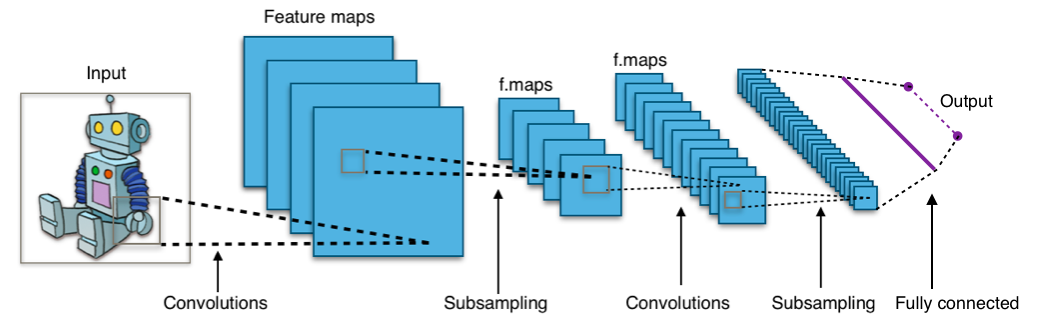
\includegraphics[width=0.8\linewidth]{6.png}
	\caption{A typical CNN model}
\end{figure}

\qquad We are going to get training data from Internet and generate by ourself. Also, we plan to use Tensorflow as our development tool. 

\section{Project Scope}
\subsection{Project Goal and Task}
\begin{enumerate}[1.]
	\item Implement image in-painting algorithm. When it is given an image and a chosen area, it can remove the object in the area and inpaint the image.
	\item Implement the CNN model, and get data to train this modle. Finally, we plan to get a better result than traditional algorithm.
	\item Transform the implementation code to frond end application, such as Andorid application and web page application. We are going to do a perfect demo in the presentation. 
\end{enumerate}
\subsection{Project Costs}
\qquad In our project, there is no too much money cost needed. But in our CNN model, it may need a lot of time to train the neural network model. Also, it may need GPU to decrease the training time cost.
\subsection{Project Deadline}
\qquad The concrete time schedule is shown in section 6. 

\qquad The deadline of this project is 1/10/2017.
\subsection{Possible problem}
There are some possible problem that we may meet when do this project.
\begin{enumerate}[1.]
	\item There is no previous people who do image in-painting using CNN model. So it is really a big challenge for us. We plan to try our best to get a great CNN model about image in-painting, but it may have some problem. But we will try out best to solve it.
	\item It may need too much calculation that can not be done on embedded system such as Android phone. But we will try our best to optimize it. 
\end{enumerate}
\section{Benefits}
\qquad In our daily life, there may be something that added to image for some intention, or something that exists on the image that we want to remove. Our software will help them solve these problem. In our plan, we will make an application that can inpaint the image with a novel algorithm and we can not find and trace. 
\section{Methodology}
\begin{table}[H]
	\centering
	\begin{tabular}{|c|c|c|}
		\hline
		Major Mission & Date & Finished or Not \\
		\hline
		Paper research, UML design, Requirement analysis
		& 9/15 - 11/16& Finished \\
		\hline
		 Prototype design, Network structure design, 
		 & 11/17 - 11/30 & TODO \\
		\hline
		 Backend developement, Algorithm implementation & 12/1 - 12/14 & TODO\\
		\hline
		 Frontend implementation, UI design & 12/14 - 12/28 & TODO\\
		\hline
		 Test and refactoring & 12/28 - 1/10 & TODO\\
		\hline 
		
	\end{tabular}
\end{table}


\section{Hardware and Software Resources}
In this project, we have to deal with hardware and software resources since 
in a software development, these resources are critical.

Hardware:
\begin{enumerate}
\item 1 Android and 2 iPhone devices
\item GPU to train nerual networks
\item 3 laptops for software development
\end{enumerate}

Software:
\begin{enumerate}
\item use Python/Java as backend programming language
\item deep learning training platform: tensorflow
\item use Javascript to build frontend logic
\item use CSS/html for UI design
\end{enumerate}



\section{Task Distribution}
\begin{table}[H]
	\centering
	\begin{tabular}{|c|c|c|}
		\hline
		Student Name & Student ID & Task Assigned \\
		\hline
		Hu Hu & 5140519019 & Frontend and  backend implementation  \\
		\hline
		Yesheng Ma & 5140209064 & Backend implementation and UI design\\
		\hline
		Yikai Zou & 5140309276 & Documentation, paper research and UML design\\
		\hline
	\end{tabular}
\end{table}

\end{document}

